\section{Design}
\begin{figure}
  \centering
  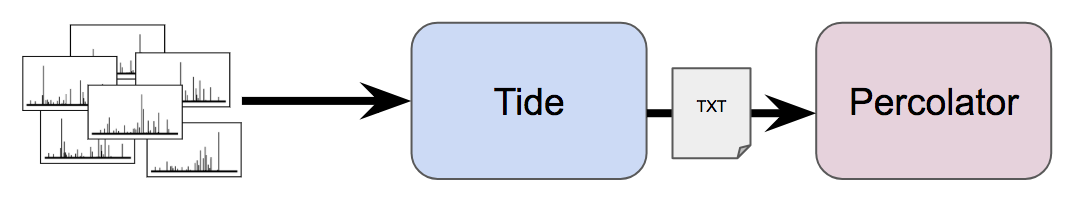
\includegraphics[scale=0.3]{serial_pipeline}
  \caption{Serial Pipeline}
  \label{fig:serial_pipeline}
\end{figure}
\begin{figure}
  \centering
  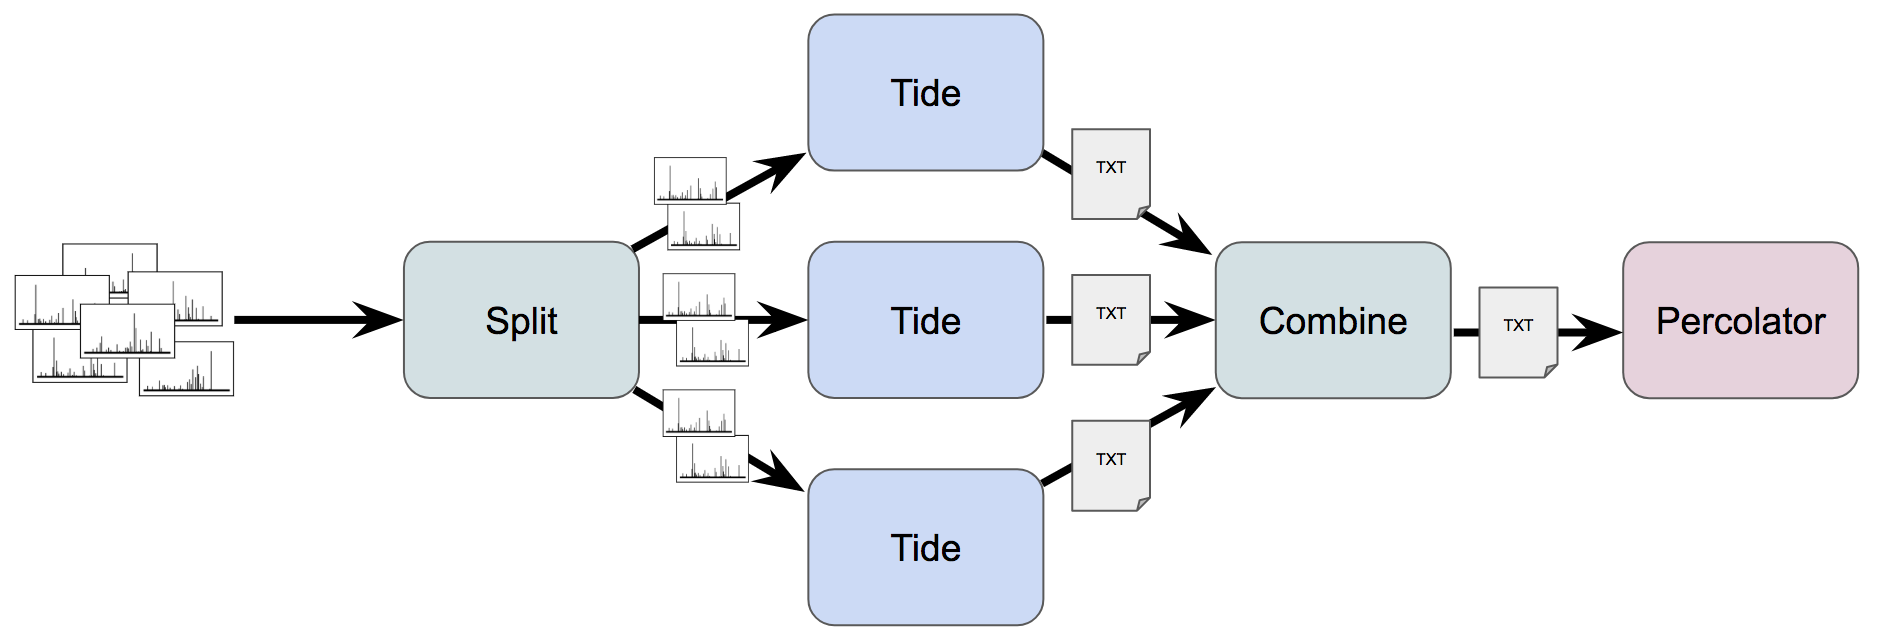
\includegraphics[scale=0.3]{lambda_pipeline}
  \caption{Lambda Pipeline}
  \label{fig:lambda_pipeline}
\end{figure}
As shown in Figure \ref{fig:serial_pipeline}, in the serial pipeline, experimental spectra is given to Tide. Tide processes the spectra and outputs the matches and these matches can be passed to Percolator.

%\\Matching the experimental spectra against theoretical spectra can be extremely slow. To speed up the process, Tide can compute index values for the theoretical spectra and use these indices to speed up the search process.\\

